\documentclass[conference]{IEEEtran}
\IEEEoverridecommandlockouts

\usepackage{cite}
\usepackage{amsmath,amssymb,amsfonts}
\usepackage{algorithmic}
\usepackage{graphicx,float}
\usepackage{textcomp}
\usepackage{xcolor}
\usepackage{fancyhdr}

\pagestyle{fancy}
\fancyhf{} 
\fancyfoot[C]{Makalah IF2211 Strategi Algoritma -- Teknik Informatika ITB -- Semester II Tahun 2025/2026}

\renewcommand{\headrulewidth}{0pt} 
\renewcommand{\footrulewidth}{0pt}
\usepackage[colorlinks=true, linkcolor=blue, urlcolor=blue, citecolor=blue]{hyperref}

\graphicspath{{images/}}
\def\BibTeX{{\rm B\kern-.05em{\sc i\kern-.025em b}\kern-.08em
    T\kern-.1667em\lower.7ex\hbox{E}\kern-.125emX}}
\begin{document}

\title{\Huge {Implementasi Algoritma \textit{Backtracking} dengan Optimasi Pemangkasan Ruang Status pada Permainan Nonogram}}

\author{
    \IEEEauthorblockN{Geraldo Artemius - 13524005}
    \IEEEauthorblockA{
        \textit{Program Studi Teknik Informatika} \\
        \textit{Sekolah Teknik Elektro dan Informatika} \\
        Institut Teknologi Bandung, Jl. Ganesha 10 Bandung 40132, Indonesia \\
        Email : 
        $^1$\textit{\href{mailto:13524005@std.stei.itb.ac.id}{13524005@std.stei.itb.ac.id}}, $^2$\textit{\href{mailto:geraldoartemius2005@gmail.com}{geraldoartemius2005@gmail.com}}
    }
}

\maketitle

\thispagestyle{fancy}

\begin{abstract}

Permainan Nonogram merupakan teka-teki logika visual termasuk NP-Complete, di mana solusi dicari dengan mewarnai sel pada \textit{grid} berdasarkan petunjuk angka. Pencarian solusi secara naif sangat tidak efisien karena kompleksitas waktu yang eksponensial seiring bertambahnya ukuran papan. Makalah ini menyajikan implementasi algoritma Runut-Balik (\textit{Backtracking}) untuk menyelesaikan permainan Nonogram secara otomatis. Untuk mengatasi banyaknya kombinasi pada ruang pencarian, diterapkan optimasi melalui pemangkasan ruang status (\textit{state space pruning}). Dalam implementasi ini, ruang status diekspansi secara bertahap, dan sebuah fungsi pembatas (\textit{bounding function}) sebagai pengevaluasi validitas konfigurasi baris dan kolom setiap kali sel diwarnai. Jika penempatan warna melanggar \textit{bounding function} seperti melebihi batas kapasitas blok atau ketidaksesuaian urutan maka simpul tersebut langsung dimatikan dan algoritma melakukan \textit{backtracking}. Algoritma ini diupayakan mencegah program untuk menelusuri cabang yang tidak valid. Penggunaan \textit{bounding function} secara signifikan mengurangi jumlah simpul di dalam pohon pencarian. Hasilnya menunjukkan bahwa algoritma Backtracking dengan optimasi pemangkasan merupakan pendekatan komputasional yang sangat efektif untuk menyelesaikan permainan Nonogram.

Kata Kunci—Nonogram, \textit{Backtracking}, Pemangkasan Ruang Status, \textit{Bounding Function}, \textit{Depth-First Search}
\end{abstract}

\section{PENDAHULUAN}
\begin{figure}[H]
    \centering
    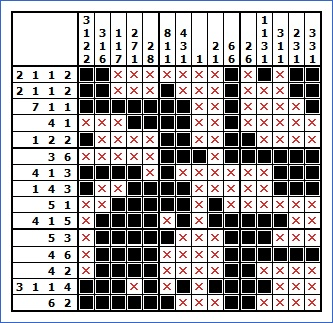
\includegraphics[width=0.55\linewidth]{example3.jpg}
    \caption{Contoh Papan Permainan Nonogram. \footnotesize\href{https://www.wastudentmath.org/pages/puzzles/nonogram}{sumber}}
    \label{fig:papan-1}
\end{figure}

Permainan Nonogram, yang juga dikenal sebagai \textit{Griddlers} atau \textit{picture cross puzzles}, merupakan permainan yang melatih kemampuan kognitif seperti memori, perhatian, dan penalaran. Tujuan utama dari permainan ini adalah mengisi papan permainan dengan warna untuk menunjukkan sebuah gambar tersembunyi. Pengisian grid ini tidak dilakukan dengan menebak secara acak, melainkan menggunakan logika deduktif berdasarkan deret angka petunjuk yang terdapat pada sisi setiap baris dan kolom.

Meskipun aturan dasarnya cukup sederhana, penyelesaian Nonogram menghadirkan tantangan komputasi yang sangat tinggi. Bagi manusia, penyelesaian \textit{puzzle} ini mengandalkan pengenalan pola visual. Namun, dari sudut pandang ilmu komputer, mencari solusi pada \textit{grid} Nonogram adalah sebuah masalah optimasi kombinatorial yang kompleks dan diklasifikasikan sebagai masalah NP-Complete. Seiring bertambahnya dimensi papan permainan, jumlah kemungkinan kombinasi warna pada kotak akan meningkat secara eksponensial, sehingga pencarian solusi secara manual atau \textit{brute force} sangat tidak efisien.

Salah satu metode yang paling sesuai untuk masalah pencarian kombinatorial adalah algoritma Runut-Balik (\textit{Backtracking}). Algoritma ini bekerja dengan membangun kandidat solusi secara bertahap dan segera melakukan proses \textit{backtracking} apabila sebuah kandidat/simpul terbukti melanggar aturan. Agar pencarian solusi dapat berjalan optimal dan tidak terjebak dalam ledakan kombinasi, algoritma ini memerlukan optimasi berupa pemangkasan ruang status (\textit{state space pruning}). Dengan menerapkan fungsi pembatas (\textit{bounding function}), algoritma dapat mendeteksi ketidaksesuaian tata letak blok warna lebih awal dan membuang cabang kemungkinan yang salah tanpa harus menelusurinya hingga akhir.

Makalah ini bertujuan untuk mengimplementasikan algoritma \textit{Backtracking} dengan mengaplikasikan teknik pemangkasan ruang status untuk menyelesaikan permainan Nonogram. Tujuan dari makalah ini adalah untuk menganalisis dan mendemonstrasikan bagaimana pembatasan ekspansi simpul pada pohon pencarian dapat mengefisienkan waktu penyelesaian masalah teka-teki gambar ini. Objektif utama dari penulisan ini terletak pada perancangan logika komputasional \textit{bounding function} yang secara selalu memvalidasi aturan baris dan kolom, sehingga menghasilkan program pencari solusi yang sistematis dan optimal.

\section{LANDASAN TEORI}
\subsection{Permainan Nonogram}
\textbf{Pengisian \textit{Grid}} \\
Dalam proses pencarian solusi, pemain dapat mengeksekusi dua jenis aksi pengisian terhadap kotak-kotak di dalam papan:
\begin{itemize}
    \item \textbf{Mode Isi ($\blacksquare$):} Aksi untuk mengisi kotak dengan warna, yang menandakan bahwa kotak tersebut adalah bagian valid dari gambar.
    \item \textbf{Mode Tandai ($\times$):} Aksi untuk memberikan tanda silang pada kotak sebagai penanda bahwa kotak tersebut dipastikan bukan bagian dari gambar.
\end{itemize}

\textbf{Aturan Angka dan Jarak (\textit{Constraints})} \\
\begin{figure}[H]
    \centering
    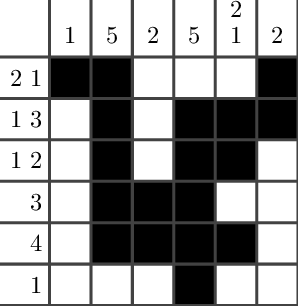
\includegraphics[width=0.5\linewidth]{contohjarak.png}
    \caption{Implementasi Jarak Pada Nonogram. \footnotesize\href{https://www.youtube.com/watch?v=DXVfgpewEK8}{sumber}}
    \label{fig:contoh-jarak}
\end{figure}
Setiap baris (horizontal) dan kolom (vertikal) pada papan, baik yang berukuran $5 \times 5$, $10 \times 10$, maupun ukuran lainnya dalam format $N\times N$, dilengkapi dengan angka petunjuk di sebelah kiri atau atas. Angka-angka ini merepresentasikan aturan yang harus dipenuhi:
\begin{itemize}
    \item \textbf{Deret Berurutan:} Angka petunjuk menunjukkan berapa banyak kotak berurutan yang harus diisi. Sebagai contoh, petunjuk "3" berarti pemain harus mengisi 3 kotak secara berurutan.
    \item \textbf{Aturan Jarak:} Ketika terdapat beberapa angka petunjuk untuk satu baris atau kolom (misalnya "1 2"), blok kotak yang diisi harus dipisahkan oleh setidaknya satu kotak kosong. Dalam contoh "1 2", pemain harus mengisi 1 kotak, memberikan jarak minimal satu kotak kosong, lalu mengisi 2 kotak berurutan.
\end{itemize}

\textbf{Strategi Deduksi} \\
Penyelesaian Nonogram tidak mengandalkan tebakan acak, melainkan menggunakan deduksi berdasarkan panjang kisi-kisi dan petunjuk angka. Sebagai contoh pada papan dengan kapasitas lebar 5 kotak:
\begin{itemize}
    \item \textbf{Kapasitas Penuh:} Jika petunjuknya adalah "5", maka seluruh 5 kotak dipastikan terisi. Jika petunjuknya adalah "2 2", berdasarkan aturan jarak wajib, susunannya dipastikan menjadi 2 kotak isi, 1 kotak kosong, dan 2 kotak isi.
    \item \textbf{Irisan Pasti (\textit{Overlapping}):} Jika petunjuknya adalah "4", terdapat dua kemungkinan posisi (dimulai dari kiri atau kanan). Namun, tiga kotak di bagian tengah akan selalu terisi pada kedua kemungkinan tersebut. Maka kotak-kotak ini dapat langsung diisi sebagai langkah awal deduksi.
\end{itemize}
Penandaan kotak yang dipastikan kosong menggunakan $\times$ akan membantu mempersempit ruang kemungkinan, sehingga proses deduksi atau penyimpulan langkah selanjutnya menjadi lebih efisien.

\textbf{Kondisi Penyelesaian (\textit{Goal State})}
\begin{figure}[H]
    \centering
    
\includegraphics[width=0.5\linewidth]{Goal State.png}
    \caption{Contoh Mencapai Goal State. \footnotesize\href{https://www.crazygames.com/game/nonogram}{sumber}}
    \label{fig:goal-state}
\end{figure}
Kondisi penyelesaian yang valid (\textit{goal state}) tercapai apabila seluruh kotak telah dievaluasi dan diisi sehingga memenuhi semua syarat petunjuk angka di seluruh baris dan kolom. Pada saat kondisi ini terpenuhi secara serentak, konfigurasi kotak-kotak tersebut akan menampilkan sebuah karya seni piksel utuh.

\subsection{Teori Kompleksitas dan NP-Complete}
\textbf{Kompleksitas Waktu Algoritma} \\
Berdasarkan kebutuhan waktu eksekusinya, algoritma untuk menyelesaikan sebuah persoalan dibagi menjadi dua kelompok besar: algoritma waktu polinom (\textit{polynomial-time algorithms}) dan algoritma waktu non-polinom (\textit{nonpolynomial-time algorithms}). Algoritma waktu-polinom adalah algoritma yang kompleksitas waktunya dibatasi oleh fungsi polinom. Sebuah persoalan dikatakan \textit{tractable} jika ia dapat diselesaikan dalam waktu yang wajar. Sebaliknya, persoalan dikatakan \textit{intractable} jika tidak dapat diselesaikan dalam waktu yang wajar seiring dengan bertambahnya ukuran masukan. Algoritma waktu non-polinom dibatasi oleh fungsi non-polinom dan sering kali dianggap sebagai persoalan yang sulit.

\textbf{Kelas P dan NP} \\
Dalam pembahasan teori kompleksitas, batasan utamanya sering kali difokuskan pada persoalan keputusan (\textit{decision problem}), yaitu persoalan yang solusinya hanya berupa jawaban "ya" atau "tidak".
\begin{itemize}
    \item \textbf{Kelas P (\textit{Polynomial}):} Merupakan semua persoalan keputusan yang dapat dipecahkan oleh algoritma deterministik dalam waktu polinom. Semua persoalan keputusan yang dapat diselesaikan dalam waktu polinom adalah anggota himpunan P.
    \item \textbf{Kelas NP (\textit{Non-deterministic Polynomial}):} Merupakan persoalan keputusan yang dapat diselesaikan oleh algoritma non-deterministik dalam waktu polinomial (\textit{non-deterministic polynomial-time algorithm}). Ini berarti, jika diberikan sebuah kandidat solusi, kebenaran solusi tersebut dapat diverifikasi dalam waktu polinom. Setiap persoalan keputusan yang kompleksitas waktunya polinomial solusinya juga dapat diverifikasi dalam waktu polinom, sehingga kelas P adalah himpunan bagian dari NP ($P \subseteq NP$).
\end{itemize}

\begin{figure}[H]
    \centering
    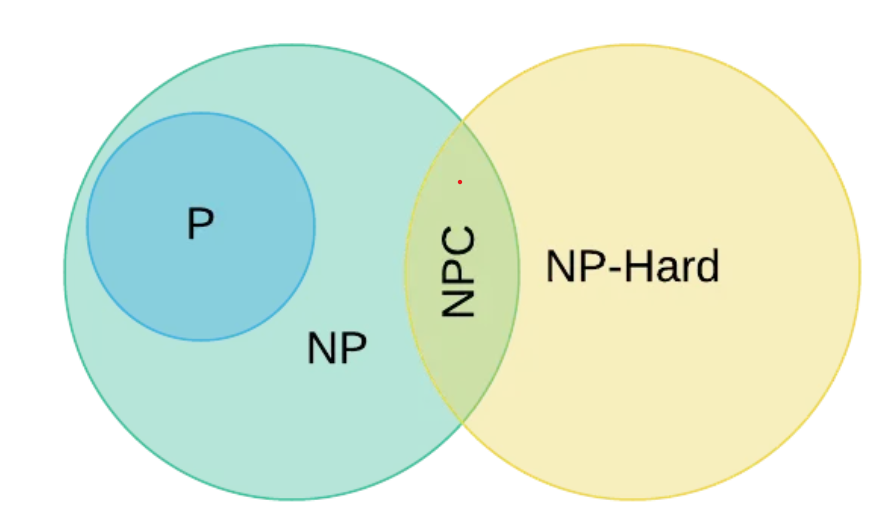
\includegraphics[width=0.5\linewidth]{pnp.png}
    \caption{Hubungan P, NP, NP-Complete, NP-Hard}
    \label{fig:pnpnpcnphard}
\end{figure}

\textbf{Kelas NP-Complete (NPC)} \\
NP-Complete (NPC) adalah himpunan persoalan NP yang paling sulit namun sangat menarik. Sebuah persoalan $X$ didefinisikan sebagai NP-Complete jika memenuhi dua syarat berikut:
\begin{enumerate}
    \item Persoalan $X$ termasuk ke dalam kelas NP.
    \item Setiap persoalan di dalam kelas NP dapat direduksi (ditransformasikan) menjadi $X$ dalam waktu polinom.
\end{enumerate}
Apabila sebuah algoritma waktu-polinom berhasil ditemukan untuk menyelesaikan satu persoalan NPC, maka seluruh persoalan di dalam kelas NP dapat dipecahkan dalam waktu polinom.

\textbf{Nonogram sebagai Masalah NP-Complete} \\
Permainan Nonogram diklasifikasikan ke dalam kategori NP-Complete. Hal ini dapat dibuktikan melalui dua parameter berikut:
\begin{itemize}
    \item \textbf{Pembuktian Kelas NP:} Jika sebuah tebakan solusi Nonogram diberikan (sebuah matriks yang telah diwarnai secara penuh), kebenaran solusi tersebut dapat diverifikasi dalam waktu polinom. Program hanya perlu melakukan iterasi satu kali pada setiap baris dan kolom untuk mencocokkannya dengan petunjuk angka.
    \item \textbf{Kompleksitas Pencarian:} Pada matriks berukuran $N \times M$, setiap kotak memiliki dua kemungkinan status (diisi atau disilang). Mencari solusi yang tepat dengan mencoba semua kombinasi secara \textit{brute force} membutuhkan waktu eksponensial. 
\end{itemize}

\subsection{Algoritma Runut-Balik (\textit{Backtracking})}

\textbf{Konsep Dasar Algoritma Runut-Balik} \\
Algoritma runut-balik merupakan perbaikan dari algoritma pencarian solusi secara \textit{exhaustive search}. Pada \textit{exhaustive search}, semua kemungkinan solusi dieksplorasi dan dievaluasi satu per satu. Sebaliknya, pada algoritma \textit{backtracking}, hanya pilihan yang mengarah ke solusi yang dieksplorasi. Pilihan yang tidak mengarah ke solusi tidak akan dipertimbangkan lagi melalui proses pemangkasan (\textit{pruning}).

\textbf{Properti Umum Algoritma} \\
Dalam merumuskan penyelesaian dengan \textit{backtracking}, terdapat tiga properti umum yang harus didefinisikan:
\begin{enumerate}
    \item \textbf{Vektor Solusi:} Solusi dari sebuah persoalan dinyatakan sebagai vektor dengan $n$-tuple: $$X = (x_1, x_2, ..., x_n)$$
    \item \textbf{Fungsi Pembangkit:} Dinyatakan sebagai fungsi $$T(x_1, x_2, ..., x_{k-1})$$ bertugas untuk membangkitkan nilai bagi $x_k$, yaitu komponen vektor solusi pada langkah ke-$k$.
    \item \textbf{Fungsi Pembatas (\textit{Bounding Function}):} Dinyatakan sebagai predikat $$B(x_1, x_2, ..., x_k)$$ yang mengembalikan nilai \textit{true} atau \textit{false}. Fungsi ini bernilai \textit{true} apabila nilai $(x_1, x_2, ..., x_k)$ mengarah ke solusi dan tidak melanggar \textit{constraints} persoalan. Jika mengembalikan nilai \textit{true}, proses pembangkitan diteruskan ke langkah $k+1$, namun jika \textit{false}, maka kandidat kombinasi tersebut dibuang/dimatikan.
\end{enumerate}

\textbf{Pohon Ruang Status (\textit{State Space Tree})} \\
\begin{figure}[H]
    \centering
    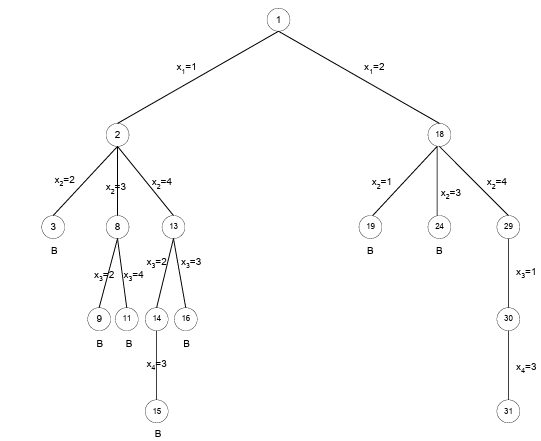
\includegraphics[width=1\linewidth]{statetree.png}
    \caption{Contoh \textit{State Space Tree} Persoalan N-Queens $4\times 4$}
    \label{fig:state-space-tree}
\end{figure}

Semua kemungkinan solusi dari persoalan (ruang solusi) diorganisasikan ke dalam sebuah struktur pohon berakar. Algoritma \textit{backtracking} pada dasarnya dapat dipandang sebagai proses pencarian di dalam pohon tersebut, bergerak dari akar menuju daun. 

Pohon ruang status memiliki tiga macam simpul, yaitu simpul akar, simpul dalam, dan simpul daun. Setiap simpul di dalam pohon ini merepresentasikan status (\textit{state}) persoalan pada tahap tertentu, sementara sisi atau cabangnya dilabeli dengan nilai-nilai penugasan variabel solusi. Sebuah solusi yang mungkin direpresentasikan oleh sebuah lintasan dari simpul akar hingga ke simpul daun. 

\textbf{Prinsip Pencarian dan Pemangkasan Ruang Status} \\
Pencarian solusi secara sistematis pada pohon ruang status dilakukan melalui tahapan berikut:
\begin{enumerate}
    \item \textbf{Pembangkitan Simpul:} Pencarian dimulai dengan membangkitkan simpul-simpul status sehingga membentuk lintasan dari akar ke daun mengikuti mekanisme pencarian \textit{Depth-First Search} (DFS). Simpul yang telah dibangkitkan dinamakan simpul hidup (\textit{live node}), dan simpul hidup yang saat ini sedang diperluas dinamakan simpul-E (\textit{Expand-node}). 
    \item \textbf{Pemangkasan (\textit{Pruning}):} Tiap kali simpul-E diperluas, lintasan solusi yang dibangun akan bertambah panjang. Jika evaluasi menunjukkan bahwa lintasan tersebut tidak mengarah ke solusi, simpul-E akan "dimatikan" menggunakan \textit{bounding function}. Statusnya berubah menjadi simpul mati (\textit{dead node}), dan algoritma secara implisit memangkas seluruh cabang simpul anaknya.
    \item \textbf{Runut-Balik (\textit{Backtrack}):} Apabila pembentukan lintasan berujung pada simpul mati, algoritma akan melakukan proses runut-balik ke simpul hidup pada aras (\textit{level}) tepat di atasnya.
    \item \textbf{Eksplorasi Lanjutan:} Dari simpul hidup tersebut, algoritma meneruskan eksplorasi dengan membangkitkan simpul anak cabang lainnya untuk dijadikan simpul-E yang baru. Proses runut-balik dan ekspansi ini berulang hingga algoritma mencapai simpul solusi atau seluruh ruang pencarian habis dievaluasi.
\end{enumerate}

\section{Perancangan dan Implementasi Algoritma}
\subsection{Pemodelan dan Representasi Data Nonogram}
\textbf{Representasi Papan Permainan (Ruang Pencarian)} \\
Papan permainan Nonogram dimodelkan sebagai matriks (array dua dimensi) berukuran $N \times M$, di mana $N$ adalah jumlah baris dan $M$ adalah jumlah kolom. Misalkan matriks ini direpresentasikan dengan variabel \texttt{board[N][M]}. Pada awal permainan (status awal atau \textit{initial state}), seluruh elemen matriks diinisialisasi dengan nilai yang menandakan bahwa kotak tersebut belum dievaluasi.

\textbf{Nilai Variabel (Sel)} \\
Setiap sel atau kotak pada koordinat $(i, j)$ di dalam matriks bertindak sebagai variabel keputusan. Dalam pendekatan runut-balik ini, domain nilai untuk setiap sel \texttt{board[i][j]} dibatasi pada tiga \textit{state}:
\begin{itemize}
    \item \texttt{0} (\textit{UNASSIGNED}): Menandakan bahwa sel masih kosong dan belum diberikan tebakan warna.
    \item \texttt{1} (\textit{FILLED}): Menandakan bahwa sel ditebak berisi blok warna.
    \item \texttt{2} (\textit{CROSSED}): Menandakan bahwa sel ditebak pasti kosong (X).
\end{itemize}

\textbf{Representasi (\textit{Clues})} \\
Petunjuk angka yang berada di luar kisi-kisi permainan bertindak sebagai himpunan (\textit{constraints}). Petunjuk ini direpresentasikan menggunakan struktur data \textit{array of lists} (atau \textit{array of vectors} dalam implementasinya). 
\begin{itemize}
    \item \texttt{rowClue[i]} menyimpan deretan angka petunjuk untuk baris ke-$i$.
    \item \texttt{colClue[j]} menyimpan deretan angka petunjuk untuk kolom ke-$j$.
\end{itemize}
Sebagai contoh, jika baris pertama memiliki petunjuk angka "1 2", maka \texttt{RowClues[0]} akan berisi himpunan nilai \texttt{\{1, 2\}}.

\textbf{Definisi Transisi Status} \\
Sebuah status (\textit{state}) didefinisikan sebagai satu konfigurasi spesifik dari matriks \texttt{board} pada waktu tertentu. Transisi dari satu status ke status lainnya di dalam pohon ruang status terjadi ketika algoritma memilih satu sel \texttt{board[i][j]} yang masih bernilai \texttt{0}, dan mencoba mengubah nilainya menjadi \texttt{1} (cabang kiri pohon) atau \texttt{2} (cabang kanan pohon). Transisi ini akan terus dilakukan hingga matriks terisi penuh dan memenuhi seluruh elemen pada \texttt{rowClue} dan \texttt{colClue}, yang menandakan tercapainya status solusi (\textit{goal state}).

\begin{table}[hbt!]
\centering
\begin{tabular}{|l|}
\hline
\textbf{Deklarasi Tipe Data dan Ruang Status} \\
\hline
\vspace{-0.5em} \\

\textbf{type} \textsf{CellState} : \textbf{enum} \{\textsf{UNASSIGNED}=0, \textsf{FILLED}=1, \textsf{CROSSED}=2\} \\
\\
\textbf{class} \textsf{Nonogram} \\
\quad \textbf{Deklarasi Atribut (private):} \\
\quad \quad $N, M$ : \textbf{integer} \textit{// $N$ baris dan $M$ kolom} \\
\quad \quad \textsf{board} : \textbf{matriks} $N \times M$ \textbf{of} \textsf{CellState} \\
\quad \quad \textsf{rowClue} : \textbf{array of list of integer} \\
\quad \quad \textsf{colClue} : \textbf{array of list of integer} \\
\vspace{-0.5em} \\
\hline
\end{tabular}
\label{tab:pseudo_nonogram}
\end{table}

\subsection{Fungsi Pembangkit}
Pada penyelesaian Nonogram, fungsi ini diimplementasikan melalui sebuah prosedur rekursif yang mengevaluasi setiap sel \texttt{board} secara sekuensial dari kiri atas hingga kanan bawah.

\textbf{Mekanisme Pemilihan Variabel} \\
Pencarian solusi dilakukan sel demi sel. Misalkan algoritma saat ini berada pada sel dengan koordinat baris $i$ dan kolom $j$. Algoritma pertama-tama akan memeriksa apakah indeks baris $i$ telah mencapai nilai $N$ (jumlah total baris). Jika $i = N$, maka seluruh sel pada matriks telah berhasil diisi, yang menandakan bahwa status solusi (\textit{goal state}) telah tercapai (kondisi basis/ \textit{base case}). Jika belum, program akan menghitung koordinat sel berikutnya, yaitu bergeser ke kanan ($j+1$), atau turun ke baris baru ($i+1$) apabila indeks $j$ telah mencapai ujung kolom.

\textbf{Pembangkitan Cabang dan \textit{Backtracking}} \\
Untuk setiap sel $(i, j)$ yang diekspansi, fungsi pembangkit akan menghasilkan dua kemungkinan status baru secara berurutan:
\begin{enumerate}
    \item \textbf{Eksplorasi Cabang Kiri (Blok Warna):} Fungsi akan mencoba \textit{assign} status \texttt{FILLED} pada \texttt{board[i][j]}. Setelah ini, (\textit{bounding function}) dipanggil untuk memvalidasi apakah penempatan blok warna tersebut tidak melanggar petunjuk angka (\textit{clues}) baris dan kolom. Jika valid, fungsi memanggil dirinya sendiri secara rekursif untuk mengekspansi sel selanjutnya.
    \item \textbf{Eksplorasi Cabang Kanan (Sel Kosong):} Apabila cabang pertama mengembalikan nilai salah, baik karena ditolak langsung oleh fungsi pembatas maupun karena menemui jalan buntu di kedalaman rekursi, algoritma akan melakukan \textit{backtracking}. Nilai \texttt{board[i][j]} diubah menjadi \texttt{CROSSED}, dan proses validasi serta pemanggilan rekursif diulang untuk status baru ini.
\end{enumerate}
Jika kedua penugasan (\texttt{FILLED} dan \texttt{CROSSED}) sama-sama menghasilkan status tidak valid atau jalan buntu, maka sel $(i, j)$ dikembalikan ke status awalnya (\texttt{UNASSIGNED}), dan fungsi akan mengembalikan nilai salah (\textit{false}) kepada pemanggil di aras atasnya untuk memicu \textit{backtracking} lebih lanjut.

\subsection{Perancangan \textit{Bounding Function}}
Fungsi ini akan mengevaluasi validitas konfigurasi matriks \texttt{board} sesaat setelah sebuah sel $(i, j)$ diberikan penugasan status baru, serta mendeteksi jalan buntu (\textit{dead end}) secepat mungkin.

Fungsi pembatas, diimplementasikan dengan \texttt{boundingFunction(i, j)}, fungsi akan  membandingkan status sel-sel pada baris ke-$i$ dan kolom ke-$j$ terhadap himpunan \textit{constraints} \texttt{rowClue[i]} dan \texttt{colClue[j]}. Sebuah simpul dinyatakan mati dan ruang statusnya dipangkas apabila memenuhi salah satu dari pelanggaran berikut:

\begin{enumerate}
    \item \textbf{Pelanggaran Penjumlahan Petunjuk:} \\
    Fungsi menghitung total akumulasi sel bernilai \texttt{FILLED} pada baris $i$ dan kolom $j$ saat ini. Jika jumlah sel \texttt{FILLED} melebihi total penjumlahan angka pada \texttt{rowClue[i]} atau \texttt{colClue[j]}, maka status tersebut dipastikan tidak valid.
    
    \item \textbf{Pelanggaran Ukuran Blok:} \\
    Algoritma menelusuri deretan sel \texttt{FILLED} yang berurutan. Jika terdapat blok warna yang panjangnya melebihi angka petunjuk (\textit{clue}) yang sedang dievaluasi pada baris atau kolom tersebut, maka simpul langsung dimatikan.
    
    \item \textbf{Pelanggaran Aturan Jarak:} \\
    Dua angka petunjuk yang berbeda mengisyaratkan adanya dua blok warna yang terpisah. Jika fungsi mendeteksi dua blok \texttt{FILLED} menyatu tanpa adanya minimal satu sel \texttt{CROSSED} atau \texttt{UNASSIGNED} di antaranya, maka konfigurasi tersebut melanggar aturan jarak dan algoritma akan memicu runut-balik.
\end{enumerate}

Apabila ketiga uji kendala di atas berhasil dilewati, maka fungsi pembatas mengembalikan nilai benar (\textit{true}), yang mengisyaratkan bahwa lintasan dari akar ke simpul saat ini masih berpotensi mengarah ke simpul solusi. Sebaliknya, jika salah satu evaluasi gagal, fungsi mengembalikan nilai salah (\textit{false}), memberitahu fungsi pembangkit bahwa status saat ini adalah jalan buntu dan harus segera dianulir.

\begin{table}[H] 
\centering
\small 
\begin{tabular}{|p{0.95\linewidth}|} 
\hline
\textbf{Pseudocode Fungsi Pembatas} \\
\hline
\vspace{-0.5em} \\ 
\textbf{function} \textsf{BoundingFunction}($row, col$ : \textbf{integer}) $\rightarrow$ \textbf{boolean} \\
\quad \textit{// 1. Evaluasi Kapasitas Maksimal (Overfill)} \\
\quad $maxAllowedRow \leftarrow$ jumlah angka petunjuk $\textsf{rowClue}[row]$ \\
\quad $curFilledRow \leftarrow$ total \textsf{FILLED} pada $\textsf{board}[row][0 \dots col]$ \\
\quad \textbf{if} $curFilledRow > maxAllowedRow$ \textbf{then} \\
\quad \quad \textbf{return false} \\
\quad \textbf{end if} \\
\\
\quad $maxAllowedCol \leftarrow$ jumlah angka petunjuk $\textsf{colClue}[col]$ \\
\quad $curFilledCol \leftarrow$ total \textsf{FILLED} pada $\textsf{board}[0 \dots row][col]$ \\
\quad \textbf{if} $curFilledCol > maxAllowedCol$ \textbf{then} \\
\quad \quad \textbf{return false} \\
\quad \textbf{end if} \\
\vspace{-0.5em} \\
\hline
\end{tabular}
\end{table}

\begin{table}[H] 
\centering
\small 
\begin{tabular}{|p{0.95\linewidth}|} 
\hline
\vspace{-0.5em} \\ 
\quad \textit{// 2. Evaluasi Ukuran Blok dan Jarak pada Baris} \\
\quad $idxRow \leftarrow 0$, $curBlockRow \leftarrow 0$ \\
\quad \textbf{for} $i \leftarrow 0$ \textbf{to} $col$ \textbf{do} \\
\quad \quad \textbf{if} $\textsf{board}[row][i] == \textsf{FILLED}$ \textbf{then} \\
\quad \quad \quad $curBlockRow \leftarrow curBlockRow + 1$ \\
\quad \quad \textbf{else if} $\textsf{board}[row][i] == \textsf{CROSSED}$ \textbf{and} $curBlockRow > 0$ \textbf{then} \\
\quad \quad \quad \textbf{if} $idxRow \ge$ ukuran($\textsf{rowClue}[row]$) \textbf{or} \\
\quad \quad \quad $curBlockRow \neq \textsf{rowClue}[row][idxRow]$ \textbf{then} \\
\quad \quad \quad \quad \textbf{return false} \\
\quad \quad \quad \textbf{end if} \\
\quad \quad \quad $idxRow \leftarrow idxRow + 1$, $curBlockRow \leftarrow 0$ \\
\quad \quad \textbf{end if} \\
\quad \textbf{end for} \\
\\
\quad \textit{// Evaluasi ujung blok terakhir} \\
\quad \textbf{if} $curBlockRow > 0$ \textbf{then} \\
\quad \quad \textbf{if} $idxRow \ge$ ukuran($\textsf{rowClue}[row]$) \textbf{or} \\
\quad \quad $curBlockRow > \textsf{rowClue}[row][idxRow]$ \textbf{then} \\
\quad \quad \quad \textbf{return false} \\
\quad \quad \textbf{end if} \\
\quad \textbf{end if} \\
\\
\quad \textit{// 3. Evaluasi Kolom (Logika serupa dengan baris)} \\
\quad \textbf{if} terdapat blok kolom tidak valid \textbf{or} melebihi batas \textbf{then} \\
\quad \quad \textbf{return false} \\
\quad \textbf{end if} \\
\\
\quad \textbf{return true} \\
\textbf{end function} \\
\vspace{-0.5em} \\
\hline
\end{tabular}
\end{table}

\subsection{\textit{Preprocessing} dan Deduksi Logis}
Meskipun algoritma \textit{backtracking} dengan fungsi pembatas mampu memangkas ruang pencarian secara signifikan, proses eksplorasi sel demi sel dari awal masih membutuhkan waktu komputasi yang besar, terutama pada matriks berukuran luas. Untuk menanggulangi hal tersebut, diimplementasikan sebuah tahap prapemrosesan (\textit{pre-processing}) yang dieksekusi satu kali sebelum algoritma pencarian utama berjalan. Tahap ini bertujuan untuk menggabungkan heuristik deduksi logis manusia dengan kecepatan komputasi mesin.

\textbf{1) Irisan Kepastian} \\
Salah satu teknik deduksi yang paling efektif dalam Nonogram adalah strategi irisan kepastian. Teknik ini mengidentifikasi sel-sel yang dipastikan bernilai \texttt{FILLED} sesuai dengan ukuran \textit{board}.

Apabila sebuah baris atau kolom dengan kapasitas panjang $L$ memiliki sebuah petunjuk angka tunggal $C$, dan nilai $C$ tersebut memenuhi syarat $C \gt \frac{L}{2}$, maka akan selalu terdapat irisan blok warna yang tumpang tindih. Secara matematis, sel-sel yang dipastikan terisi berada pada rentang indeks $j$ (dengan basis indeks 0) sebagai berikut:
\begin{equation*}
    (L - C) \le j \le (C - 1)
\end{equation*}

Sebagai contoh, pada matriks berukuran $10 \times 10$ ($L = 10$) dengan petunjuk baris $C = 9$, sel yang pasti terisi adalah dari indeks $j = (10 - 9)$ hingga $j = (9 - 1)$, yaitu indeks ke-1 sampai ke-8. Pada matriks $15 \times 15$ ($L = 15$) dengan petunjuk $C = 14$, sel yang pasti terisi berada pada rentang indeks $1$ hingga $13$.

\textbf{2) Strategi Baris Penuh} \\
Selain irisan kepastian, algoritma prapemrosesan juga mendeteksi kondisi di mana sebuah baris atau kolom memiliki konfigurasi yang pasti tanpa perlu ditebak. Kondisi ini terjadi apabila total panjang seluruh blok warna yang diisyaratkan oleh petunjuk, ditambah dengan jumlah spasi minimum yang memisahkan blok-blok tersebut, sama persis dengan kapasitas panjang baris atau kolom ($L$).

Secara matematis, misalkan sebuah baris memiliki himpunan petunjuk $C = \{c_1, c_2, \dots, c_k\}$ dengan jumlah elemen $k$. Kondisi baris penuh terpenuhi jika:
\begin{equation*}
    \left( \sum_{i=1}^{k} c_i \right) + (k - 1) = L
\end{equation*}

Sebagai contoh, pada matriks berukuran $10 \times 10$ ($L = 10$), jika terdapat petunjuk baris bernilai $\{5, 4\}$, maka total ruang yang dibutuhkan adalah $5 + 4 + (2 - 1) = 10$. Karena kebutuhan ruang sama dengan kapasitas matriks, konfigurasi ini bersifat pasti. Fungsi prapemrosesan akan langsung mengisi sel-sel tersebut secara berurutan dengan status \texttt{FILLED} dan menyisipkan \texttt{CROSSED} sebagai pemisah.

\begin{table}[H] 
\centering
\small 
\begin{tabular}{|p{0.95\linewidth}|} 
\hline
\vspace{-0.5em} \\ 
\textbf{procedure} \textsf{PreProcess}() \\
\quad \textit{// 1. Evaluasi Setiap Baris} \\
\quad \textbf{for} $i \leftarrow 0$ \textbf{to} $N - 1$ \textbf{do} \\
\quad \quad $L \leftarrow M$ \textit{// Kapasitas baris} \\
\quad \quad \textit{// Strategi Irisan Kepastian (Overlapping)} \\
\quad \quad \textbf{if} ukuran($\textsf{rowClue}[i]$) $== 1$ \textbf{then} \\
\quad \quad \quad $C \leftarrow \textsf{rowClue}[i][0]$ \\
\quad \quad \quad \textbf{if} $C > L / 2$ \textbf{then} \\
\quad \quad \quad \quad \textbf{for} $j \leftarrow (L - C)$ \textbf{to} $(C - 1)$ \textbf{do} \\
\quad \quad \quad \quad \quad $\textsf{board}[i][j] \leftarrow \textsf{FILLED}$ \\
\quad \quad \quad \quad \textbf{end for} \\
\quad \quad \quad \textbf{end if} \\
\quad \quad \textbf{end if} \\
\quad \quad \textit{// Strategi Baris Penuh (Perfect Match)} \\
\quad \quad $sumClue \leftarrow$ jumlah total elemen pada $\textsf{rowClue}[i]$ \\
\quad \quad $minSpace \leftarrow$ ukuran($\textsf{rowClue}[i]$) - 1 \\
\quad \quad \textbf{if} $(sumClue + minSpace) == L$ \textbf{then} \\
\quad \quad \quad $j \leftarrow 0$ \\
\quad \quad \quad \textbf{for each} $c$ \textbf{in} $\textsf{rowClue}[i]$ \textbf{do} \\
\quad \quad \quad \quad \textit{// Isi blok warna} \\
\quad \quad \quad \quad \textbf{for} $k \leftarrow 1$ \textbf{to} $c$ \textbf{do} \\
\quad \quad \quad \quad \quad $\textsf{board}[i][j] \leftarrow \textsf{FILLED}$ \\
\quad \quad \quad \quad \quad $j \leftarrow j + 1$ \\
\quad \quad \quad \quad \textbf{end for} \\
\quad \quad \quad \quad \textit{// Sisipkan spasi pembatas} \\
\quad \quad \quad \quad \textbf{if} $j < L$ \textbf{then} \\
\quad \quad \quad \quad \quad $\textsf{board}[i][j] \leftarrow \textsf{CROSSED}$ \\
\quad \quad \quad \quad \quad $j \leftarrow j + 1$ \\
\quad \quad \quad \quad \textbf{end if} \\
\quad \quad \quad \textbf{end for} \\
\quad \quad \textbf{end if} \\
\quad \textbf{end for} \\
\quad \textit{// 2. Evaluasi Setiap Kolom} \\
\quad \textit{// (Menerapkan strategi Irisan Kepastian dan Baris Penuh} \\
\quad \textit{// secara identik pada setiap indeks kolom } $j \leftarrow 0 \dots M-1$) \\
\textbf{end procedure} \\
\vspace{-0.5em} \\
\hline
\end{tabular}
\label{tab:pseudo_preprocess}
\end{table}

\subsection{Implementasi \textit{Backtracking}}
Algoritma berada di dalam sebuah fungsi rekursif \textsf{solve} yang bertugas menelusuri pohon ruang status sel demi sel secara sekuensial. 

Fungsi ini menyatukan seluruh komponen yang telah dirancang sebelumnya. Alur kerjanya mencakup:
\begin{enumerate}
    \item \textbf{Pengecekan Kondisi Basis:} Jika indeks baris telah mencapai akhir matriks ($N$), pencarian dihentikan dan program mengembalikan nilai benar (\textit{true}) yang menandakan solusi telah ditemukan.
    \item \textbf{Integrasi Prapemrosesan:} Fungsi mengecek apakah sel saat ini sudah diisi oleh tahap prapemrosesan. Jika sel tidak bernilai \texttt{UNASSIGNED}, fungsi tidak akan mencoba menebak, melainkan langsung melakukan rekursi ke sel berikutnya.
    \item \textbf{Pembangkitan dan Pemangkasan (\textit{Pruning}):} Fungsi membangkitkan cabang pertama dengan menugaskan status \texttt{FILLED}. Jika lolos dari \textit{bounding function}, pencarian dilanjutkan. Jika gagal, fungsi membangkitkan cabang kedua (\texttt{CROSSED}).
    \item \textbf{Runut-Balik (\textit{Backtrack}):} Jika kedua cabang menghasilkan jalan buntu (\textit{false}), fungsi menganulir tebakan dengan mengembalikan status sel menjadi \texttt{UNASSIGNED}, lalu memicu runut-balik ke kedalaman rekursi sebelumnya.
\end{enumerate}

\begin{table}[H] 
\centering
\small 
\begin{tabular}{|p{0.95\linewidth}|} 
\hline
\textbf{Pseudocode Solve} \\
\hline
\vspace{-0.5em} \\ 
\textbf{function} \textsf{Solve}($row, col$ : \textbf{integer}) $\rightarrow$ \textbf{boolean} \\
\quad \textit{// 1. Kondisi Basis: Berhasil mencapai batas akhir baris} \\
\quad \textbf{if} $row == N$ \textbf{then} \textbf{return true} \\
\\
\quad \textit{// Menghitung koordinat sel berikutnya} \\
\quad $nextRow, nextCol \leftarrow$ hitung\_koordinat\_sel\_berikutnya($row, col$) \\
\\
\quad \textit{// 2. Integrasi Prapemrosesan: Lompat jika sudah terisi} \\
\quad \textbf{if} $\textsf{board}[row][col] \neq \textsf{UNASSIGNED}$ \textbf{then} \\
\quad \quad \textbf{return} \textsf{Solve}($nextRow, nextCol$) \\
\quad \textbf{end if} \\
\\
\quad \textit{// 3. Pembangkitan Cabang Pertama (Blok Warna)} \\
\quad $\textsf{board}[row][col] \leftarrow \textsf{FILLED}$ \\
\quad \textbf{if} \textsf{BoundingFunction}($row, col$) $==$ \textbf{true} \textbf{then} \\
\quad \quad \textbf{if} \textsf{Solve}($nextRow, nextCol$) $==$ \textbf{true} \textbf{then} \\
\quad \quad \quad \textbf{return true} \\
\quad \quad \textbf{end if} \\
\quad \textbf{end if} \\
\quad \textit{// 4. Pembangkitan Cabang Kedua (Sel Kosong/Silang)} \\
\quad $\textsf{board}[row][col] \leftarrow \textsf{CROSSED}$ \\
\quad \textbf{if} \textsf{BoundingFunction}($row, col$) $==$ \textbf{true} \textbf{then} \\
\quad \quad \textbf{if} \textsf{Solve}($nextRow, nextCol$) $==$ \textbf{true} \textbf{then} \\
\quad \quad \quad \textbf{return true} \\
\quad \quad \textbf{end if} \\
\quad \textbf{end if} \\
\quad \textit{// 5. Jalan Buntu (Runut-balik / Backtrack)} \\
\quad $\textsf{board}[row][col] \leftarrow \textsf{UNASSIGNED}$ \\
\quad \textbf{return false} \\
\textbf{end function} \\

\vspace{-0.5em} \\
\hline
\end{tabular}
\end{table}

\section{HASIL DAN PEMBAHASAN}
\subsection{\textit{Test Case} 1}
\textbf{$10 \times10$}
\begin{figure}[H]
    \centering
    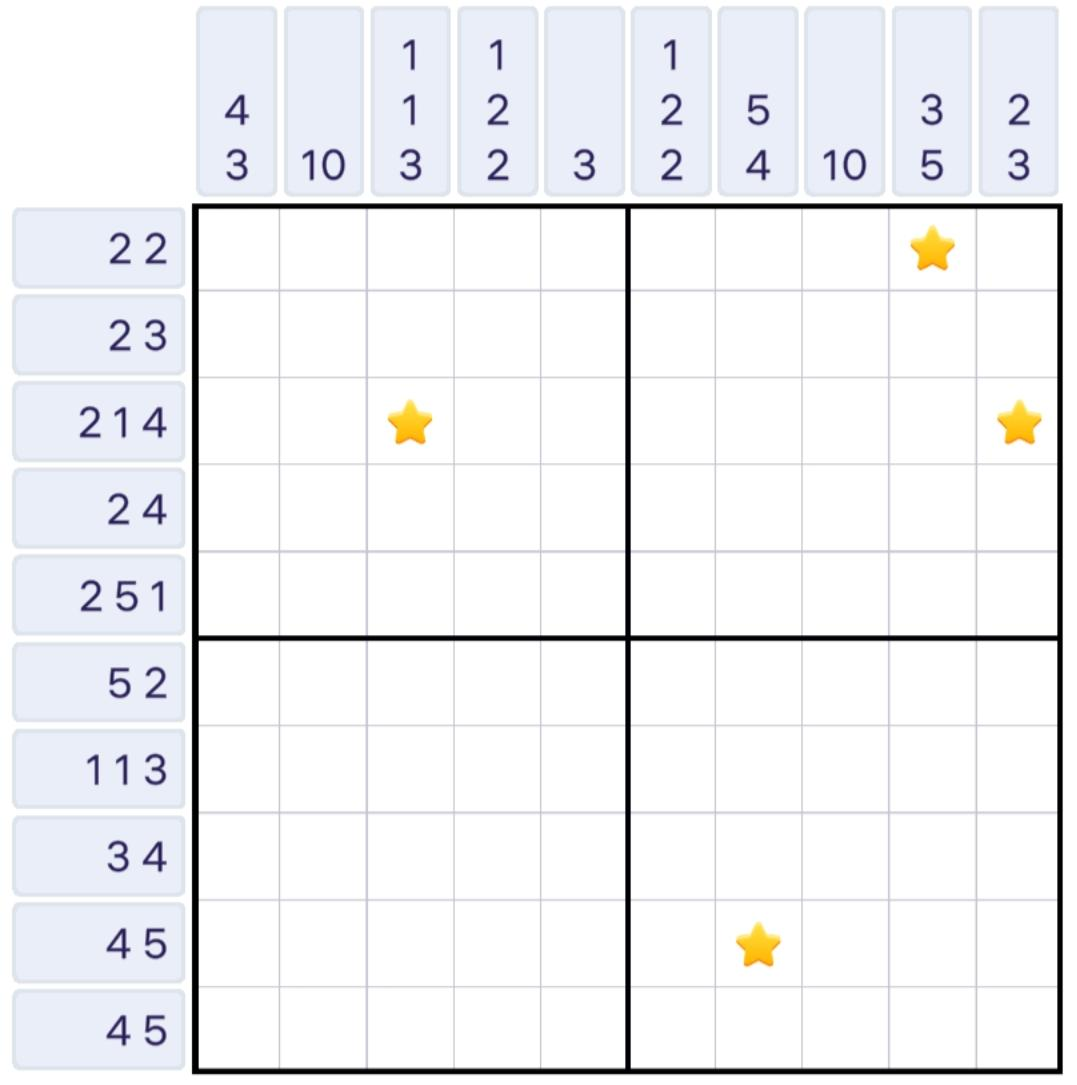
\includegraphics[width=0.5\linewidth]{test1game.png}
    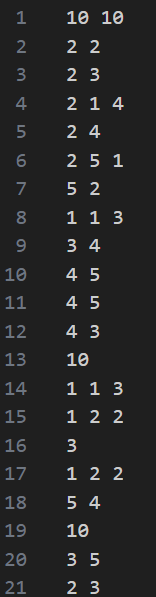
\includegraphics[width=0.2\linewidth]{images/test1Code.png}
    \caption{Test Case 1 dari Game Nonogram.}
    \label{fig:testcase-1}
\end{figure}

\textbf{Hasil Program}
\begin{figure}[H]
    \centering
    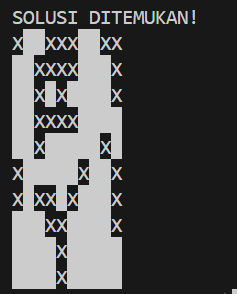
\includegraphics[width=0.5\linewidth]{result1Code.png}
    \caption{Hasil Input \textit{Test Case} 1 pada Program (Mencapai Goal State)}
    \label{fig:testcase-1-result}
\end{figure}
\begin{figure}[H]
    \centering
    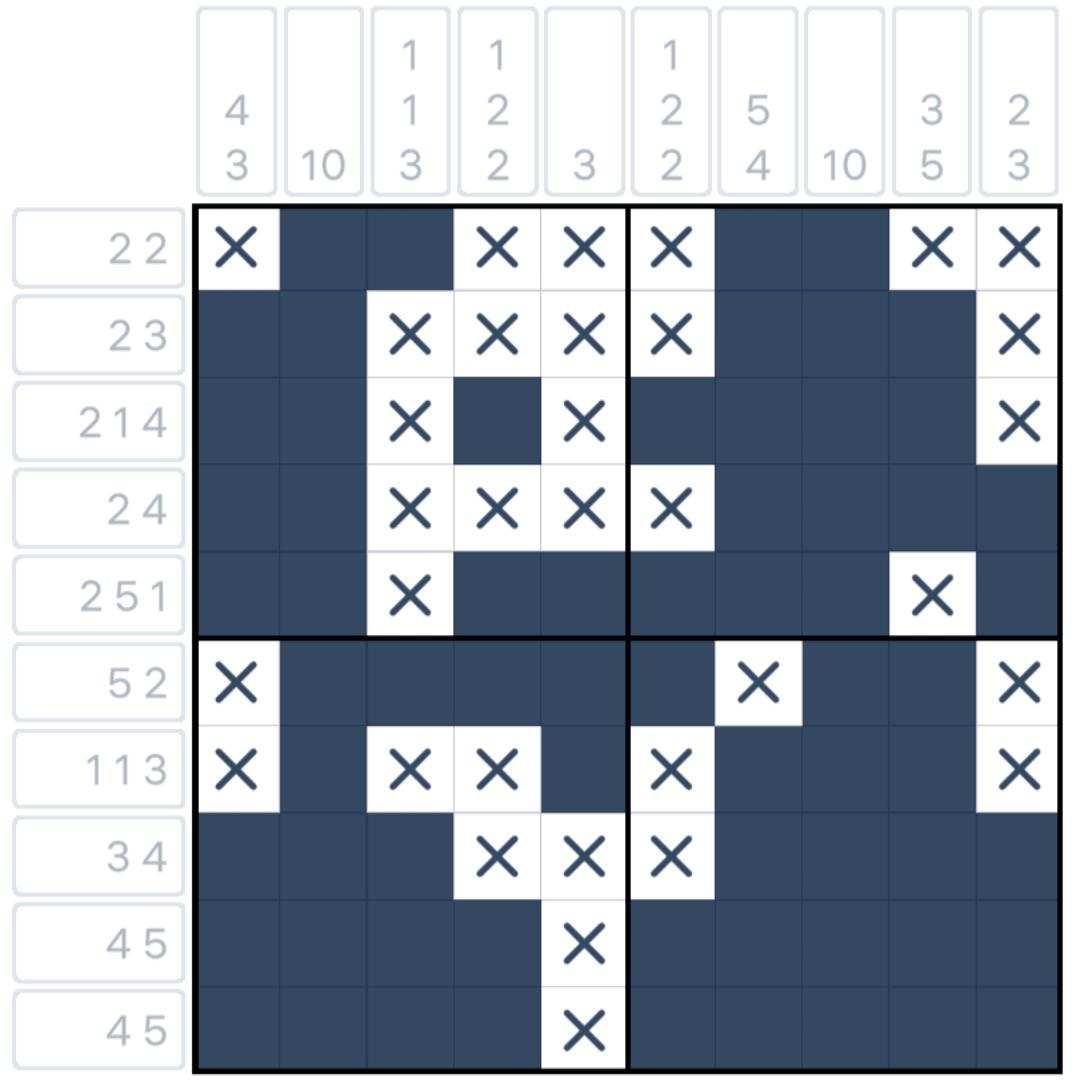
\includegraphics[width=0.5\linewidth]{test1GameResult.png}
    \caption{Solusi \textit{Test Case }1 di Game Nonogram}
    \label{fig:testcase-1-gameresult}
\end{figure}
Program membaca masukan berekstensi \texttt{.txt} yang berisi ukuran papan dan (\textit{clue}) permainan. Dua nilai pertama pada berkas masukan menyatakan ukuran papan, yaitu $10 \times 10$. Selanjutnya, program membaca petunjuk untuk setiap baris, dimulai dari baris pertama dengan \textit{clue} ``2 2'', baris kedua ``2 3'', hingga baris kesepuluh ``4 5''. Setelah seluruh petunjuk baris dibaca, program melanjutkan pembacaan petunjuk untuk setiap kolom, dimulai dari kolom pertama dengan \textit{clue} ``4 3'' hingga kolom kesepuluh ``2 3''.

Fig. 7 menunjukkan hasil eksekusi program menggunakan \textit{test case} 1. Solusi yang dihasilkan oleh program sesuai dengan solusi referensi permainan nonogram yang ditunjukkan pada Fig. 8 yang merupakan solusi asli pada permainan Nonogram. Kesesuaian tersebut menunjukkan bahwa algoritma \textit{backtracking} berhasil menemukan konfigurasi papan yang memenuhi seluruh \textit{clue} baris dan kolom.

\subsection{\textit{Test Case} 2}
$15\times 15$

\begin{figure}[H]
    \centering
    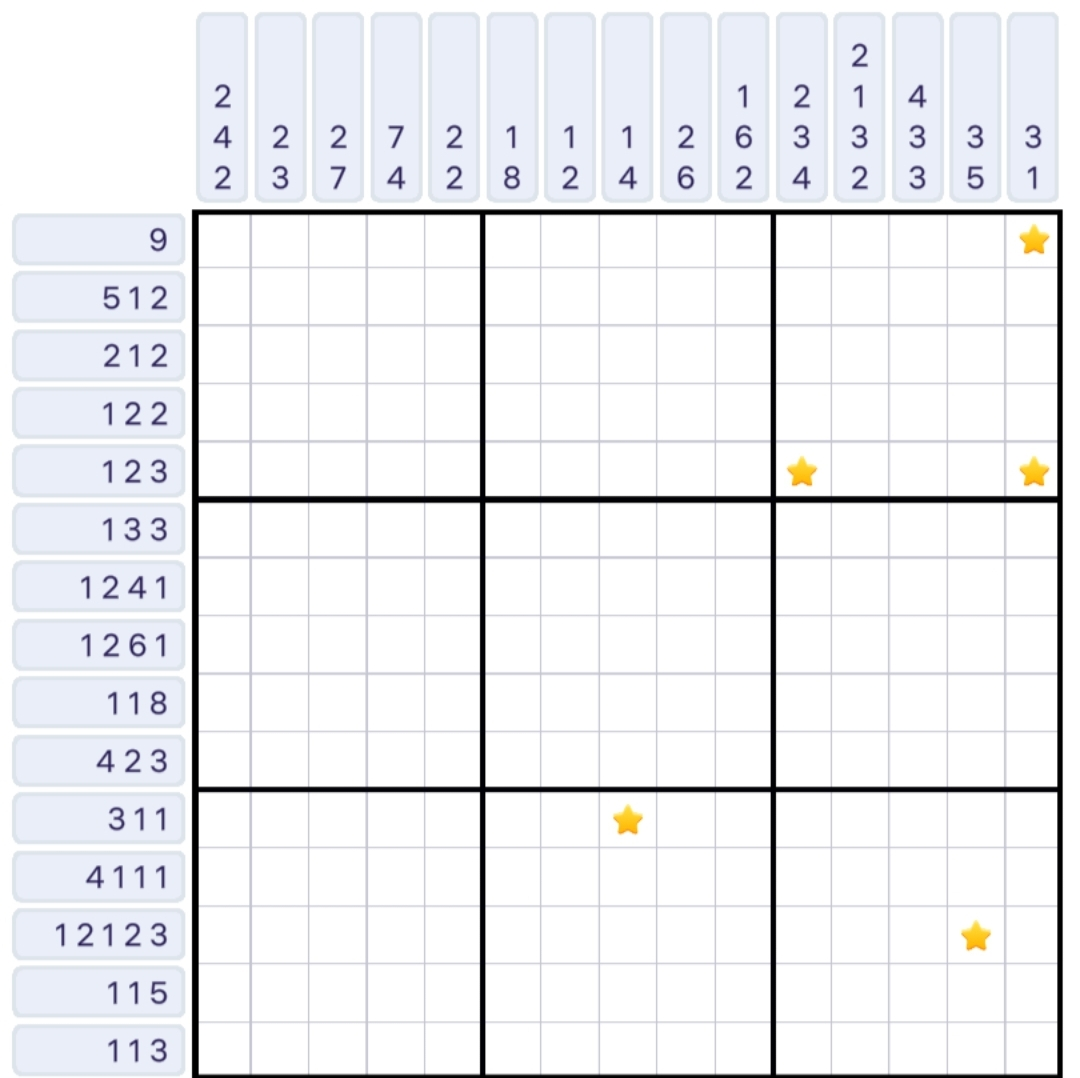
\includegraphics[width=0.5\linewidth]{images/test2Game.png}
    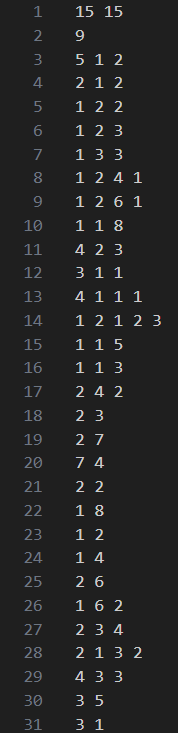
\includegraphics[width=0.2\linewidth]{images/test2Code.png}
    \caption{\textit{Test Case} 2 dari Game Nonogram}
    \label{fig:testcase-2}
\end{figure}

\begin{figure}[H]
    \centering
    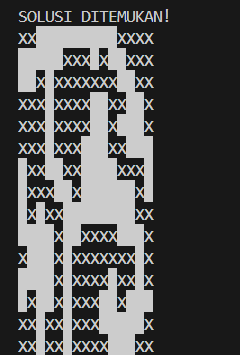
\includegraphics[width=0.4\linewidth]{test2CodeResult.png}
    \caption{Hasil Input \textit{Test Case} 2 pada Program (Mencapai Goal State)}
    \label{fig:testcase-2-result}
\end{figure}

\begin{figure}
    \centering
    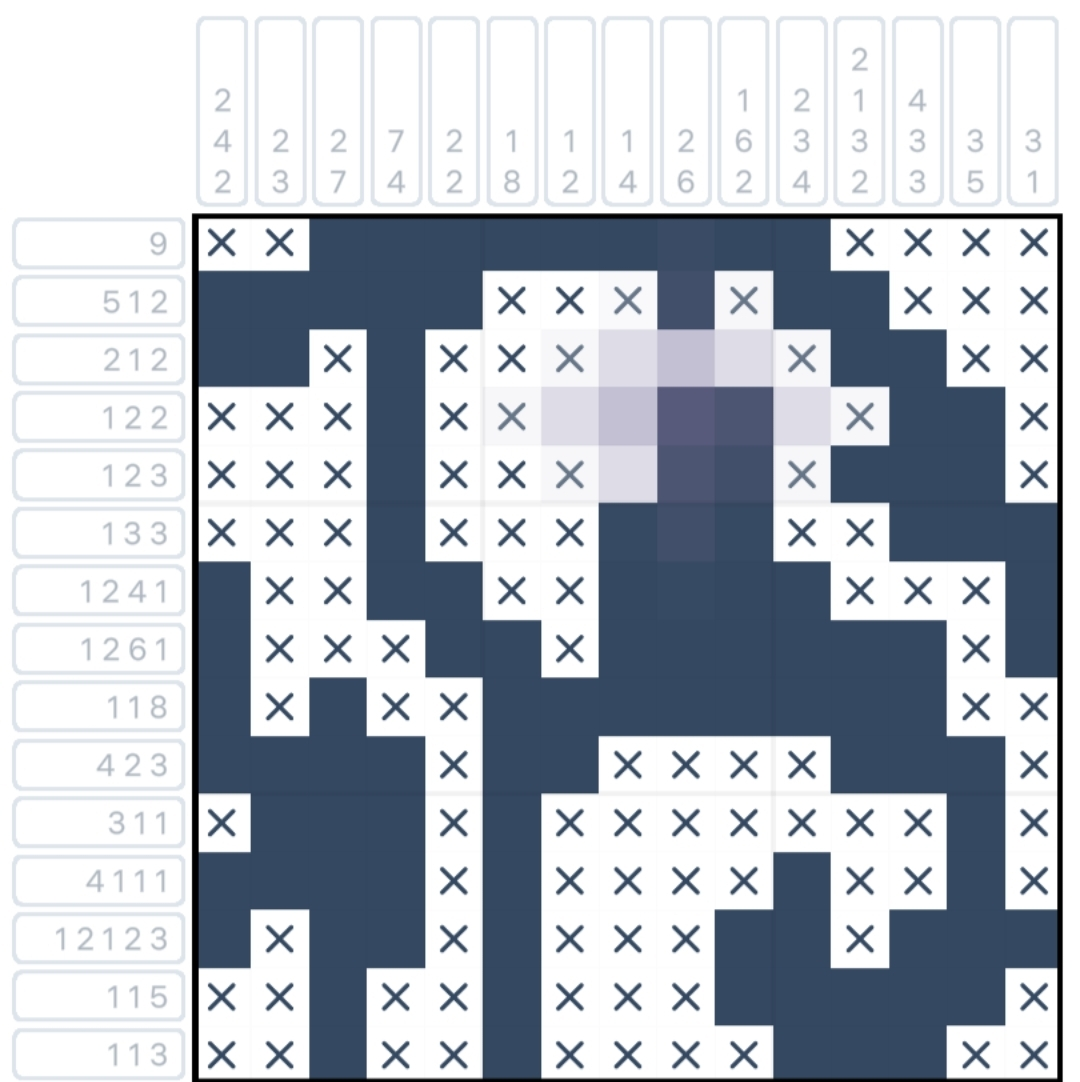
\includegraphics[width=0.5\linewidth]{images/test2GameResult.png}
    \caption{Solusi \textit{Test Case} 2 di Game Nonogram}
    \label{fig:testcase-2-gameresult}
\end{figure}

Pada \textit{test case} 2, program diuji menggunakan papan berukuran $15 \times 15$. Dibandingkan dengan \textit{test case} 1, ukuran papan yang lebih besar menghasilkan ruang pencarian yang lebih luas. Meskipun demikian, melalui mekanisme pencarian rekursif dan proses \textit{backtracking}, algoritma berhasil menemukan konfigurasi papan yang memenuhi seluruh \textit{clue} yang diberikan. Hasil eksekusi program ditunjukkan pada Fig. 10.

Berdasarkan hasil yang diperoleh, solusi yang dihasilkan identik dengan solusi asli permainan Nonogram yang ditunjukkan pada Fig. 11. Kesesuaian tersebut menunjukkan bahwa algoritma \textit{backtracking} tetap mampu menemukan solusi yang benar meskipun ukuran papan dan kompleksitas permasalahan meningkat. Dengan demikian, hasil pengujian pada \textit{test case }2 semakin memperkuat bahwa program dapat menyelesaikan permainan Nonogram secara akurat.

\section{KESIMPULAN}

Algoritma \textit{backtracking} dapat secara efektif digunakan untuk mencari solusi pada teka-teki logika Nonogram, sebuah persoalan yang secara komputasional diklasifikasikan ke dalam kelas \textit{NP-Complete}. Dengan menerapkan fungsi pembatas (\textit{bounding function}) pada setiap tahap ekspansi pohon ruang status, pemangkasan (\textit{pruning}) terhadap cabang-cabang yang tidak valid dapat dilakukan secepat mungkin sebelum memicu ekspansi jalan tidak valid yang lebih dalam. 

Meskipun persoalan \textit{NP-Complete} pada dasarnya memiliki ruang pencarian yang tumbuh secara eksponensial, hasil implementasi mengindikasikan bahwa algoritma \textit{backtracking} berbasis \textit{pruning} memberikan pendekatan yang sederhana dan efektif untuk penyelesaian Nonogram. Tujuan dari makalah ini adalah untuk memperbaiki proses penyelesaian teka-teki Nonogram, dari yang semula hanya mengandalkan komputasi tebakan buta (\textit{brute-force}) yang tidak konsisten, menjadi sebuah eksekusi yang konsisten dan cerdas dalam mencapai solusi akhir yang optimal.

\section{APENDIKS}
GitHub : \href{https://github.com/GeraldoA07/Nonogram-Backtracking-Solver}{https://github.com/GeraldoA07/Nonogram-Backtracking-Solver}

Youtube : \href{https://youtu.be/juz-4aWNsVw}{https://youtu.be/juz-4aWNsVw}

\section{UCAPAN TERIMA KASIH}
Penulis mengucapkan terima kasih yang sebesar-besarnya kepada Dr. Ir. Rinaldi Munir, M.T., atas dedikasi beliau dalam mengajar dan membimbing mata kuliah IF2211 Strategi Algoritma. Penulis juga sangat mengapresiasi dukungan serta dorongan semangat dari keluarga dan teman-teman selama proses penyelesaian makalah ini. Akhir kata, penulis memanjatkan puji syukur kepada Tuhan Yang Maha Esa atas segala rahmat dan karunia-Nya yang senantiasa memberikan kekuatan di sepanjang perjalanan penulisan ini. 

\begin{thebibliography}{00}
\bibitem{b1} R. Munir, ``Strategi Algoritma 2025-2026,'' Sekolah Teknik Elektro dan Informatika, Institut Teknologi Bandung. [Online]. Available: \url{https://informatika.stei.itb.ac.id/~rinaldi.munir/Stmik/2025-2026/stima25-26.htm}. [Accessed: Jun. 13, 2026].

\bibitem{b2} Collepic, ``Permainan Nonogram,'' Collepic.net. [Online]. Available: \url{https://collepic.net/}. [Accessed: Jun. 13, 2026].

\bibitem{b3} J. M. Buades Rubio, A. Jaume-i-Capó, D. López González, and G. Moyà Alcover, ``Solving nonograms using neural networks,'' \textit{Entertainment Computing} (Elsevier). [Online]. Available: \url{https://www.sciencedirect.com/science/article/pii/S187595212400020X}. [Accessed: Jun. 13, 2026].

\bibitem{b4} K. Sandvick, ``NP Completeness in Nonograms.'' [Online]. Available: \url{https://kelbybsandvick.github.io/pdf/NPProblemPaper.pdf}. [Accessed: Jun. 13, 2026].

\bibitem{b5} R. A. Oosterman, ``Complexity and solvability of Nonogram puzzles''. [Online]. Available: \url{https://fse.studenttheses.ub.rug.nl/15287/1/Master_Educatie_2017_RAOosterman.pdf}. [Accessed: Jun. 13, 2026].
\end{thebibliography}

\section*{PERNYATAAN}
Dengan ini saya menyatakan bahwa makalah yang saya tulis ini adalah benar-benar hasil karya saya sendiri, bukan merupakan saduran atau terjemahan dari karya orang lain, dan bukan merupakan tindakan plagiasi.

\begin{flushright}
Bandung, 13 Juni 2026


\includegraphics[width=0.4\linewidth]{images/ttd.png}

Geraldo Artemius \\
13524005
\end{flushright}

\end{document}
